\documentclass[memoire.tex]{subfiles}

\chapter*{Introduction}

\section*{Le Big Data}

La démocratisation des ordinateurs et l'avènement du WEB 2.0 ont entraîné une
digitalisation de nos connaissances. Aujourd'hui, 95\% de celles-ci sont numérisées et
la production de données est en constante évolution. Notre société produit
quotidiennement 2.5 exaoctets de données (l'équivalent de 90 années de vidéos, ou 2,5 millions de téraoctets) et en 2020 il est estimé que 35 zettaoctets seront produits (1 zettaoctet = 1000 exaoctets). Les réseaux sociaux et les objets connectés participent grandement à cette augmentation considérable du volume de données.

On caractérise le domaine du Big Data à l'aide de cinq facteurs appelé les 5V du Big Data~\cite{5V} (Figure \ref{5V-schema}).

\begin{figure}[!h]
	\centering 
	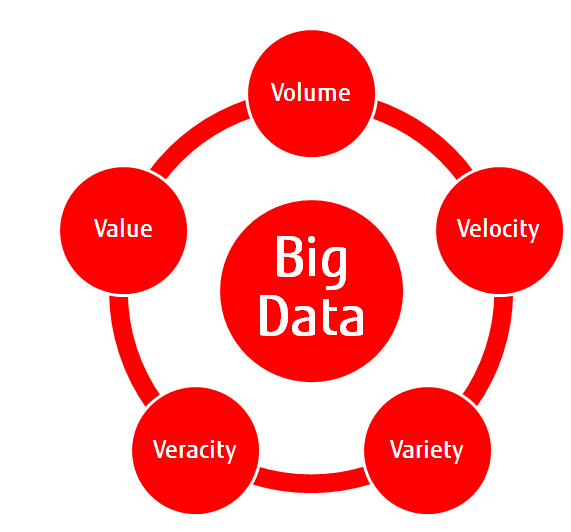
\includegraphics[scale=0.33]{img/5V.png}
	\caption{Schéma des 5V du Big Data}
	\label{5V-schema}
\end{figure}

\begin{itemize}
\item \textbf{Le volume} décrit la quantité de données générée. Il s'agit donc de la possibilité de gérer une masse de données créées quotidiennement. Par exemple, Facebook stocke aujourd'hui plus de 250 milliards d'images.
\item \textbf{La vélocité} représente la vitesse à laquelle les données arrivent. Un des meilleurs exemples pour représenter la vélocité est l'ajout de vidéos sur la plateforme Youtube. En effet, chaque minute, ce sont pas moins de 400 heures de vidéos qui sont uploadées sur la plateforme.
\item \textbf{La variété} correspond aux diverses natures que peuvent avoir les données. Par exemple, Twitter stocke du texte, des images, des fichiers vidéo, des métadonnées, etc.
\item \textbf{La véracité} met en avant la dimension qualitative nécessaire au bon fonctionnement des outils Big Data. Lorsque les données ne sont pas qualitatives, il n'est pas possible de les traiter et de s'en servir correctement.
\item \textbf{La valeur} est la plus importante des 5V. Les données auquel on s'intéresse doivent avoir une valeur réelle pour que les analyses que l'on veut effectuer ne soient pas fossés. Il est donc important de trier les données avant leur exploitation.
\end{itemize}


\section*{Quand peut-on utiliser le Big Data ?}

Le Big Data étant aujourd'hui "à la mode", c'est-à-dire que tout le monde en entend parler et donc veut aussi l'utiliser. Le problème étant que le Big Data n'est pas toujours la solution idéale pour les applications que l'on souhaite réaliser. En effet, le Big Data a été créer dans les cas où une seule machine n'est plus suffisante pour les opérations que vous avez besoin d'effectuer. Par exemple, si vos traitements de données s'effectuent sans aucun problème sur votre machine et que votre base de données n'a aucun souci de performance en étant installée sur une seule machine, il n'y a pas de réel intérêt pour vous de passer à une architecture Big Data. Dans le cas où une seule machine n'est plus suffisante pour vos besoins, avant de passer à une architecture Big Data vous pouvez essayer d'améliorer votre machine en changeant ses composants. Vous pouvez aussi essayer de rendre certaines parties de votre code asynchrones, afin d'améliorer les performances de votre code et de répartir son exécution au mieux sur votre machine. C'est ce qu'on appelle la mise à l'échelle verticale, c'est la première étape avant de passer à la mise à l'échelle horizontale ({\ref{a:architecture-repartie}}) qui est l'un des atouts principaux du Big Data. Une fois toutes ces étapes appliquées, si votre architecture n'arrive toujours pas à suivre le rythme voulu, cela veut dire que votre application est propice à l'utilisation d'une architecture Big Data.
Comme vous venez de le voir, ce n'est malheureusement pas possible de définir une limite chiffrée pour définir quand l'utilisation du Big Data est requise. Cette limite peut varier en fonction du format des données reçues, de la complexité des traitements effectués sur les données, etc. Bien évidement dans certains cas l'utilisation du Big Data est évidente (Exemple: des plateformes comme YouTube et Facebook), mais dans le cas ou vous n'avez encore jamais fait de Big Data et que vous n'avez pas un nombre de données immense, il est préférable de ne pas se diriger tout de suite vers le Big Data.
